\section{Bitcoin ownership} \label{sec:BitcoinOwnership}

\subsection{General} \label{sec:OwnershipGeneral}
Bitcoin utilizes two cryptographic primitives to realize a secure and decentralized transaction authorization system. Firstly, it employs asymmetric cryptography for (i) identification and (ii) authentication of recipients, as well as to (iii) ensure integrity of regular transactions. More precisely, the public key of a public/private keypair is used to identify a particular recipient, whereas the private key is used to create a signature for both transaction authentication and integrity.~\\

\noindent
Secondly, the proof of work protocol is used to (i) regulate coin supply, (ii) reward miners for transaction processing and (iii) ensure block integrity. In the mining process all regular transactions of users and a special coinbase transaction created by the miner are processed by solving the proof of work problem. It is important to note that while the authenticity and integrity of regular transactions is ensured by the previously discussed signature scheme, the integrity of coinbase transactions is assured by the proof of work puzzle. In the following the exact application of these primitives will be described with the help of Fig. \ref{fig:TransactionChain}.

\vspace{-5pt}
\begin{figure}[htbp]
\centering
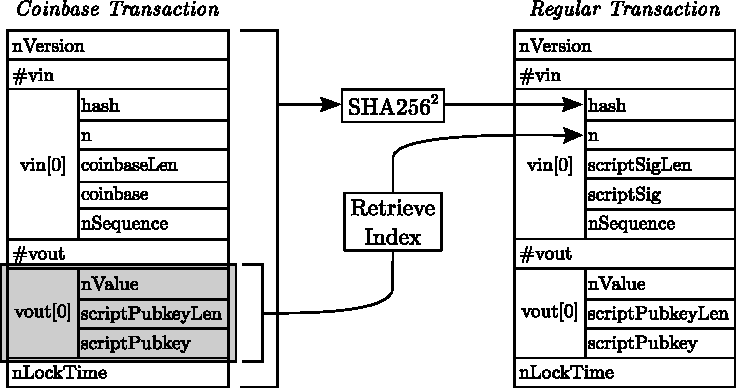
\includegraphics[scale=1]{Images/Ownership.pdf}

\caption{Bitcoin Transaction Chain}
\label{fig:TransactionChain}
\end{figure}
\vspace{-10pt}

\noindent
To begin with, Bitcoins are introduced into the system with coinbase transactions (see Sect. \ref{sec:CoinbaseTransactions}). In it the miner specifies one or more transaction outputs (\textit{vout}), defining the amounts and destinations to which the freshly created coins are to be transferred. He identifies each destination by including a public key or a derived form of it in the public key script field (\textit{scriptPubkey}). As discussed above, the integrity of the coinbase transaction is ensured by the computational hardness of the proof of work problem.~\\

\noindent
Next, when the miner intends to spend his reward, he creates a regular transaction, references it to the specific output of the coinbase transaction and provides a signature in the signature script field (\textit{scriptSig}). Since the signature is computed over the complete transactions (see Sect. \ref{sec:Signatures}), control of the private key corresponding to the referenced public key is proven and integrity of the transaction is guaranteed. This chain is continued indefinitely and logged publicly in the blockchain to keep track of all Bitcoins within the system at all times.


\subsection{Script} \label{sec:Script}
Script is a stack-based, Turing-incomplete language designed specifically for the Bitcoin protocol. A script is essentially a set of instructions\footnote{See \textit{https://en.bitcoin.it/wiki/Script} for complete reference.} that are processed left to right. Script is used to encode two components - a challenge script and a response script:

\begin{itemize}
\item[-] A challenge script (see \textit{scriptPubkey} field) is part of a transaction output and specifies under which conditions it can be claimed.
\item[-] A response script (see \textit{scriptSig} field) is part of a transaction input and is used to prove that the referenced transaction output can be rightfully claimed.
\end{itemize}

\noindent
For a given transaction, each transaction input is verified by first evaluating \textit{scriptSig}, then copying the resulting stack and finally evaluating \textit{scriptPubkey} of the referenced transaction output. If during the evaluation no failure is triggered and the final top stack element yields true, then the ownership has been successfully verified.~\\

\noindent
Although Script is very comprehensive and allows one to construct intricate conditions under which coins can be claimed, much of its functionality is currently disabled in the reference implementation and only a restricted set of standard script templates is accepted. These are \textit{Pay-to-Pubkey} (P2PK), \textit{Pay-to-PubkeyHash} (P2PKH), \textit{Pay-to-ScriptHash} (P2SH), \textit{Multisig} and \textit{Nulldata}. In the next section, the structure of these standard transaction types will be discussed.~\\


\clearpage
\enlargethispage{2\baselineskip}
\subsection{Standard Transaction Types} \label{sec:StandardTxTypes}
\vspace{6pt}

\subsubsection{Pay-to-Pubkey (P2PK)} \label{sec:P2PK}
The structure of the challenge and response scripts of a Pay-to-Pubkey transaction are depicted below in Fig. \ref{fig:P2PubStructure}. Note that operations in a script are written as \texttt{OP\_X}, where \texttt{OP} stands for operation and \texttt{X} is an abbreviation of the operation's function. For example, in Fig. \ref{fig:P2PubStructure} \texttt{CHECKSIG} stands for signature verification.

\vspace{-10pt}
\begin{figure}[htbp]

\begin{Verbatim}[fontsize==\relsize{-4}, frame=single]  
scriptPubkey: <pubkey> OP_CHECKSIG
scriptSig:    <signature>
\end{Verbatim}

\vspace{-15pt}
\caption{Pay-to-Pubkey Structure}
\label{fig:P2PubStructure}
\end{figure}
\vspace{-10pt}

\noindent
In a Pay-to-Pubkey transaction the sender transfers Bitcoins directly to the owner of a public key. He specifies in the challenge script the public key (\textit{pubkey}) and one requirement that the claimant has to prove:
\begin{enumerate}[label=\arabic*), leftmargin=1cm]
\item Knowledge of the private key corresponding to the public key.
\end{enumerate}

\noindent
To do so, the claimant creates a response script containing only a signature. The scripts are then evaluated as depicted in Table \ref{tab:P2Pub1} and \ref{tab:P2Pub2}. The signature and the public key are pushed onto the stack and evaluated. Note that the signature is computed as described in Sect. \ref{sec:Signatures}.


\begin{table}
\begin{minipage}{\textwidth}

\centering
\begin{tabular}{| m{95pt} | m{145pt} | m{100pt} |} \hline
\textbf{Stack} & \textbf{Remaining Script} & \textbf{Description} \\ \hline \hline

\vspace{8pt}
\begin{BVerbatim}[fontsize==\relsize{-4}]
Empty
\end{BVerbatim} 
\vspace{4pt}
&
\vspace{8pt}
\begin{BVerbatim}[fontsize==\relsize{-4}]
<signature>
\end{BVerbatim} 
\vspace{4pt}
&
The signature is pushed on the stack.\\ \hline

\vspace{8pt}
\begin{BVerbatim}[fontsize==\relsize{-4}]
<signature>
\end{BVerbatim} 
\vspace{4pt}
&
\vspace{8pt}
\begin{BVerbatim}[fontsize==\relsize{-4}]
Empty
\end{BVerbatim} 
\vspace{4pt}
&
Final state after evaluating \textit{scriptSig}. \\ \hline

\end{tabular}
\vspace{5pt}
\caption{Pay-to-Pubkey \textit{scriptSig} Execution}
\label{tab:P2Pub1}

\vspace{15pt}

\begin{tabular}{| m{95pt} | m{145pt} | m{100pt} |}
\hline
\textbf{Stack} & \textbf{Remaining Script} & \textbf{Description} \\ \hline \hline

\vspace{8pt}
\begin{BVerbatim}[fontsize==\relsize{-4}]
<signature>
\end{BVerbatim}
\vspace{4pt}
&
\vspace{8pt}
\begin{BVerbatim}[fontsize==\relsize{-4}]
<pubkey> OP_CHECKSIG
\end{BVerbatim} 
\vspace{4pt}
&
State after copying the stack of the signature script evaluation. The public key is pushed on the stack.\\ \hline	

\vspace{8pt}
\begin{BVerbatim}[fontsize==\relsize{-4}]
<pubkey>
<signature>
\end{BVerbatim}
\vspace{4pt}
&
\vspace{8pt}
\begin{BVerbatim}[fontsize==\relsize{-4}]
OP_CHECKSIG
\end{BVerbatim} 
\vspace{4pt}
&
The signature is verified for the top two stack elements and the result is pushed on the stack.\\ \hline	


\vspace{8pt}
\begin{BVerbatim}[fontsize==\relsize{-4}]
True
\end{BVerbatim}
\vspace{4pt}
&
\vspace{8pt}
\begin{BVerbatim}[fontsize==\relsize{-4}]
Empty
\end{BVerbatim} 
\vspace{4pt}
&
Final state after evaluating \textit{scriptPubkey}. \\ \hline

\end{tabular}
\vspace{5pt}
\caption{Pay-to-Pubkey \textit{scriptPubkey} Execution}
\label{tab:P2Pub2}

\end{minipage}
\end{table}

\clearpage
\subsubsection{Pay-to-PubkeyHash (P2PKH)} \label{sec:P2PKH}
The structure of the challenge and response scripts of a Pay-to-PubkeyHash transaction can be seen below in Fig. \ref{fig:P2PubHashStructure}.

\vspace{-10pt}
\begin{figure}[ht!]

\begin{Verbatim}[fontsize==\relsize{-4}, frame=single]  
scriptPubkey: OP_DUP OP_HASH160 <pubkeyHash> OP_EQUALVERIFY OP_CHECKSIG
scriptSig:    <signature> <pubkey>	
\end{Verbatim}

\vspace{-15pt}
\caption{Pay-to-PubkeyHash Structure}
\label{fig:P2PubHashStructure}
\end{figure}
\vspace{-10pt}

\noindent
In a Pay-to-PubkeyHash transaction the sender transfers Bitcoins to the owner of a P2PKH address (see Sect. \ref{sec:Address-P2PKH}). He specifies in the challenge script the public key hash (\textit{pubkeyHash}) of the Bitcoin address (depicted in Fig. \ref{fig:BitcoinAddress-P2PKH}) and two requirements that the claimant has to prove:

\begin{enumerate}[label=\arabic*), leftmargin=1cm]
\item Knowledge of the public key corresponding to \textit{pubkeyHash}.
\item Knowledge of the private key corresponding to the public key.
\end{enumerate}

\noindent
To do so, the claimant creates a response script containing a signature and a public key. The scripts are then evaluated as depicted in Table \ref{tab:P2PubHash1} and \ref{tab:P2PubHash2}. First, it is verified if the public key (\textit{pubkey}) corresponds to the public key hash (\textit{pubkeyHash}) and then whether the signature is valid. The signature is computed as described in Sect. \ref{sec:Signatures}.~\\


\begin{table}[!ht]
  
\begin{minipage}{\textwidth}

\centering
\begin{tabular}{| m{95pt} | m{145pt} | m{100pt} |}
\hline
\textbf{Stack} & \textbf{Remaining Script} & \textbf{Description} \\ \hline \hline

\vspace{8pt}
\begin{BVerbatim}[fontsize==\relsize{-4}]
Empty
\end{BVerbatim} 
\vspace{4pt}
&
\vspace{8pt}
\begin{BVerbatim}[fontsize==\relsize{-4}]
<signature> <pubkey>
\end{BVerbatim} 
\vspace{4pt}
&
The signature and the public key are pushed on the stack. \\ \hline


\vspace{8pt}
\begin{BVerbatim}[fontsize==\relsize{-4}]
<pubkey>
<signature>
\end{BVerbatim} 
\vspace{4pt}
&
\vspace{8pt}
\begin{BVerbatim}[fontsize==\relsize{-4}]
Empty
\end{BVerbatim} 
\vspace{4pt}
&
Final state after evaluating \textit{scriptSig}. \\ \hline

\end{tabular}
\vspace{5pt}
\caption{Pay-to-PubkeyHash \textit{scriptSig} Execution}
\label{tab:P2PubHash1}

\vspace{15pt}

\centering
\begin{tabular}{| m{95pt} | m{145pt} | m{100pt} |}
\hline
\textbf{Stack} & \textbf{Remaining Script} & \textbf{Description} \\ \hline \hline

\vspace{8pt}
\begin{BVerbatim}[fontsize==\relsize{-4}]
<pubkey>
<signature>
\end{BVerbatim}
\vspace{4pt}
&
\vspace{8pt}
\begin{BVerbatim}[fontsize==\relsize{-4}]
OP_DUP OP_HASH160 <pubkeyHash>
OP_EQUALVERIFY OP_CHECKSIG
\end{BVerbatim} 
\vspace{4pt}
&
State after copying the stack of the signature script evaluation. The top stack element is duplicated.\\ \hline


\vspace{8pt}
\begin{BVerbatim}[fontsize==\relsize{-4}]
<pubkey>
<pubkey>
<signature>
\end{BVerbatim}
\vspace{4pt}
&
\vspace{8pt}
\begin{BVerbatim}[fontsize==\relsize{-4}]
OP_HASH160 <pubkeyHash>
OP_EQUALVERIFY OP_CHECKSIG
\end{BVerbatim} 
\vspace{4pt}
&
The top stack element is first hashed with SHA256 and then with RIPEMD160.\\ \hline


\vspace{8pt}
\begin{BVerbatim}[fontsize==\relsize{-4}]
<pubkeyHashNew>
<pubkey>
<signature>
\end{BVerbatim}
\vspace{4pt}
&
\vspace{8pt}
\begin{BVerbatim}[fontsize==\relsize{-4}]
<pubkeyHash> OP_EQUALVERIFY
OP_CHECKSIG
\end{BVerbatim} 
\vspace{4pt}
&
The public key hash is pushed on the stack.\\ \hline

	
\vspace{8pt}
\begin{BVerbatim}[fontsize==\relsize{-4}]
<pubkeyHash>
<pubkeyHashNew>
<pubkey> 
<signature>
\end{BVerbatim}
\vspace{4pt}
&
\vspace{8pt}
\begin{BVerbatim}[fontsize==\relsize{-4}]
OP_EQUALVERIFY OP_CHECKSIG
\end{BVerbatim} 
\vspace{4pt}
&
Equality of the top two stack elements is checked. If it evaluates to true then execution is continued. Otherwise it fails.\\ \hline


\vspace{8pt}
\begin{BVerbatim}[fontsize==\relsize{-4}]
<pubkey>
<signature>
\end{BVerbatim}
\vspace{4pt}
&
\vspace{8pt}
\begin{BVerbatim}[fontsize==\relsize{-4}]
OP_CHECKSIG
\end{BVerbatim} 
\vspace{4pt}
&
The signature is verified for the top two stack elements.\\ \hline


\vspace{8pt}
\begin{BVerbatim}[fontsize==\relsize{-4}]
True
\end{BVerbatim}
\vspace{4pt}
&
\vspace{8pt}
\begin{BVerbatim}[fontsize==\relsize{-4}]
Empty
\end{BVerbatim} 
\vspace{4pt}
&
Final state after evaluating \textit{scriptPubkey}.\\ \hline

\end{tabular}
\vspace{5pt}
\caption{Pay-to-PubkeyHash \textit{scriptPubkey} Execution}
\label{tab:P2PubHash2}

\end{minipage}
\end{table}

\clearpage
\subsubsection{Pay-to-ScriptHash (P2SH)} \label{sec:P2SH}
The structure of the challenge and response scripts of a Pay-to-ScriptHash transaction is depicted below in Fig. \ref{fig:P2ScriptHashStructure}.

\vspace{-10pt}
\begin{figure}[htbp]

\begin{Verbatim}[fontsize==\relsize{-4}, frame=single]  
scriptPubkey: OP_HASH160 <scriptHash> OP_EQUAL
scriptSig:    <signatures> {serializedScript}
\end{Verbatim}

\vspace{-15pt}
\caption{Pay-to-ScriptHash Structure}
\label{fig:P2ScriptHashStructure}
\end{figure}
\vspace{-10pt}

\noindent
In a Pay-to-ScriptHash transaction the sender transfers Bitcoins to the owner of a P2SH Bitcoin address (see Sect. \ref{sec:Address-P2SH}). He specifies in the challenge script the serialized script hash (\textit{scriptHash}) of the Bitcoin address (depicted in Fig. \ref{fig:BitcoinAddress-P2SH}) and one requirement that the claimant has to prove:

\begin{enumerate}[label=\arabic*), leftmargin=1cm]
\item Knowledge of the redemption script \textit{serializedScript} corresponding to\\ \textit{scriptHash}.
\end{enumerate}

\noindent
To do so, the claimant creates a response script containing one or more signatures and the serialized redemption script \textit{serializedScript}. Note that unlike in any other standard transaction type the responsibility of supplying the conditions for redeeming the transaction is shifted from the sender to the redeemer. The redeemer may specify any conditions in the redemption script \textit{serializedScript} conforming to standard transaction types. For example, he may define a standard Pay-to-Pubkey transaction as a Pay-to-ScriptHash transaction as follows:

\vspace{-10pt}
\begin{figure}[htbp]

\begin{Verbatim}[fontsize==\relsize{-4}, frame=single]  
scriptPubkey: OP_HASH160 <scriptHash> OP_EQUAL
scriptSig:    <signatures> {<pubkey> OP_CHECKSIG}
\end{Verbatim}

\vspace{-15pt}
\caption{P2SH Pay-to-PublicKey Structure}
\label{fig:P2ScriptHashStructure-P2PK}
\end{figure}
\vspace{-10pt}

\noindent
Due to the nested nature of this transaction type, the script evaluation requires an additional validation step. First, it is verified whether the redemption script (\textit{serializedScript}) is consistent with the redemption script hash (\textit{scriptHash}) and then the transaction is evaluated using the redemption script as \textit{scriptPubkey}. The evaluation is depicted in Table \ref{tab:P2ScriptHash1}, \ref{tab:P2ScriptHash2} and \ref{tab:P2ScriptHash3}.

\clearpage

\begin{table}[!ht]  
\begin{minipage}{\textwidth}

\centering
\begin{tabular}{| m{105pt} | m{135pt} | m{100pt} |}
\hline
\textbf{Stack} & \textbf{Remaining Script} & \textbf{Description} \\ \hline \hline

\vspace{8pt}
\begin{BVerbatim}[fontsize==\relsize{-4}]
Empty
\end{BVerbatim} 
\vspace{4pt}
&
\vspace{8pt}
\begin{BVerbatim}[fontsize==\relsize{-4}]
<signature>
{<pubkey> OP_CHECKSIG}
\end{BVerbatim} 
\vspace{4pt}
&
The signature and the redemption script are pushed on the stack. \\ \hline


\vspace{8pt}
\begin{BVerbatim}[fontsize==\relsize{-4}]
{<pubkey> OP_CHECKSIG}
<signature>
\end{BVerbatim} 
\vspace{4pt}
&
\vspace{8pt}
\begin{BVerbatim}[fontsize==\relsize{-4}]
Empty
\end{BVerbatim} 
\vspace{4pt}
&
Final state after evaluating \textit{scriptSig}. \\ \hline

\end{tabular}
\vspace{5pt}
\caption{Pay-to-ScriptHash \textit{scriptSig} Execution}
\label{tab:P2ScriptHash1}


\vspace{15pt}


\centering
\begin{tabular}{| m{105pt} | m{135pt} | m{100pt} |}
\hline
\textbf{Stack} & \textbf{Remaining Script} & \textbf{Description} \\ \hline \hline

\vspace{8pt}
\begin{BVerbatim}[fontsize==\relsize{-4}]
{<pubkey> OP_CHECKSIG}
<signature>
\end{BVerbatim} 
\vspace{4pt}
&
\vspace{8pt}
\begin{BVerbatim}[fontsize==\relsize{-4}]
OP_HASH160 <scriptHash>
OP_EQUAL
\end{BVerbatim} 
\vspace{4pt}
&
State after copying the stack of the signature script evaluation. The top stack element is first hashed with SHA256 and then with RIPEMD160.\\ \hline


\vspace{8pt}
\begin{BVerbatim}[fontsize==\relsize{-4}]
<scriptHashNew>
<signature>
\end{BVerbatim} 
\vspace{4pt}
&
\vspace{8pt}
\begin{BVerbatim}[fontsize==\relsize{-4}]
<scriptHash> OP_EQUAL
\end{BVerbatim} 
\vspace{4pt}
&
The redemption script hash is pushed on the stack.\\ \hline


\vspace{8pt}
\begin{BVerbatim}[fontsize==\relsize{-4}]
<scriptHash>
<scriptHashNew>
<signature>
\end{BVerbatim} 
\vspace{4pt}
&
\vspace{8pt}
\begin{BVerbatim}[fontsize==\relsize{-4}]
OP_EQUAL
\end{BVerbatim} 
\vspace{4pt}
&
Equality of the top two stack elements is checked. The result of the evaluation is pushed on the stack.\\ \hline


\vspace{8pt}
\begin{BVerbatim}[fontsize==\relsize{-4}]
True
<signature>
\end{BVerbatim} 
\vspace{4pt}
&
\vspace{8pt}
\begin{BVerbatim}[fontsize==\relsize{-4}]
Empty
\end{BVerbatim} 
\vspace{4pt}
&
Final state after evaluating \textit{scriptPubkey}.\\ \hline

\end{tabular}
\vspace{5pt}
\caption{Pay-to-ScriptHash \textit{scriptPubkey} Execution}
\label{tab:P2ScriptHash2}
\end{minipage}
\end{table}

\vspace{-10pt}

\noindent
For the additional validation step the stack after \textit{scriptSig} execution (see Table \ref{tab:P2ScriptHash1}) is copied, the top stack element is popped and used as the script. The state now resembles the beginning of a standard Pay-to-Pubkey transaction evaluation (see Table \ref{tab:P2Pub2}).

\begin{table}[!h]  
	
	\centering
	\begin{tabular}{| m{105pt} | m{135pt} | m{100pt} |}
		\hline
		\textbf{Stack} & \textbf{Remaining Script} & \textbf{Description} \\ \hline \hline
		
		\vspace{8pt}
\begin{BVerbatim}[fontsize==\relsize{-4}]
<signature>
\end{BVerbatim} 
		\vspace{4pt}
		&
		\vspace{8pt}
\begin{BVerbatim}[fontsize==\relsize{-4}]
<pubkey> OP_CHECKSIG
\end{BVerbatim} 
		\vspace{4pt}
		&
		Initial state of supplementary validation step.\\ \hline
		
		\dots & \dots & \dots \\ \hline
	\end{tabular}
	
\vspace{5pt}
\caption{Pay-to-ScriptHash Supplementary Validation}
\label{tab:P2ScriptHash3}
\end{table}


\clearpage
\subsubsection{Multisig} \label{sec:Multisig}
The structure of the challenge and response scripts of a Multisig transaction is depicted below in Fig. \ref{fig:P2Multisig}.

\vspace{-10pt}
\begin{figure}[htbp]

\begin{Verbatim}[fontsize==\relsize{-4}, frame=single]  
scriptPubkey: m <pubkey 1> ... <pubkey n> n OP_CHECKMULTISIG
scriptSig:    OP_0 <signature 1> ... <signature m>
\end{Verbatim}

\vspace{-15pt}
\caption{Multisig Structure}
\label{fig:P2Multisig}
\end{figure}
\vspace{-10pt}

\noindent
In a Multisig transaction the sender transfers Bitcoins to the owner of \textit{m}-of-\textit{n} public keys. He specifies in the challenge script \textit{n} public keys (\textit{pubkey 1..n}) and a requirement that the claimant has to prove:

\begin{enumerate}[label=\arabic*), leftmargin=1cm]
\item Knowledge of at least \textit{m} private keys corresponding to the public keys.
\end{enumerate}

\noindent
To do so, the claimant creates a response script containing at least \textit{m} signatures in the same order of appearance as the public keys. Note that due to an off-by-one error {\tt OP\_CHECKMULTISIG} pops one too many elements off the stack and it is therefore required to prepend the response script with a zero data push {\tt OP\_0}. The script is then evaluated as depicted in Table \ref{tab:P2Multisig1} and \ref{tab:P2Multisig2}. First, the signatures are pushed on the stack, followed by the number of required signatures \textit{m}, the public keys and the number of public keys \textit{n}.~\\

\noindent
The bounds for a standard Multisig transaction are $1 \leq m \leq n \leq 3$, whereas for a P2SH Multisig transaction they are variable. The upper bound for a P2SH Multisig transaction is restricted by both the allowed size of the signature script \textit{scriptSig} (500 bytes) and the allowed size of the serialized script \textit{serializedScript} (520 bytes). It is therefore possible to create e.g. a 1-of-12 P2SH Multisig transaction with compressed public keys or a 4-of-5 P2SH Multisig transaction with compressed public keys. Note that the maximum size of the signature script field (\textit{scriptSig}) will be increased in the next major release to 1650 bytes, thus allowing even bigger P2SH Multisig transactions.

\begin{table}[!ht]  
\begin{minipage}{\textwidth}

\centering
\begin{tabular}{| m{95pt} | m{145pt} | m{100pt} |}

\hline
\textbf{Stack} & \textbf{Remaining Script} & \textbf{Description} \\ \hline \hline

\vspace{8pt}
\begin{BVerbatim}[fontsize==\relsize{-4}]
Empty
\end{BVerbatim} 
\vspace{4pt}
&
\vspace{8pt}
\begin{BVerbatim}[fontsize==\relsize{-4}]
OP_0 <signature 1> ...
<signature m>
\end{BVerbatim} 
\vspace{4pt}
&
The signatures are pushed on the stack.\\ \hline

\vspace{8pt}
\begin{BVerbatim}[fontsize==\relsize{-4}]
<signature m>
...
<signature 1>
OP_0
\end{BVerbatim} 
\vspace{4pt}
&
\vspace{8pt}
\begin{BVerbatim}[fontsize==\relsize{-4}]
Empty
\end{BVerbatim} 
\vspace{4pt}
&
Final state after evaluating \textit{scriptSig}. \\ \hline

\end{tabular}
\vspace{5pt}
\caption{Multisig \textit{scriptSig} Execution}
\label{tab:P2Multisig1}


\vspace{15pt}


\begin{tabular}{| m{95pt} | m{145pt} | m{100pt} |}
\hline
\textbf{Stack} & \textbf{Remaining Script} & \textbf{Description} \\ \hline \hline

\vspace{8pt}
\begin{BVerbatim}[fontsize==\relsize{-4}]
<signature m>
...
<signature 1>
OP_0
\end{BVerbatim}
\vspace{4pt}
&
\vspace{8pt}
\begin{BVerbatim}[fontsize==\relsize{-4}]
m <pubkey 1> ... <pubkey n> n
OP_CHECKMULTISIG
\end{BVerbatim} 
\vspace{4pt}
&
State after copying the stack of the signature script evaluation. The public keys are pushed on the stack.\\ \hline	

\vspace{8pt}
\begin{BVerbatim}[fontsize==\relsize{-4}]
n
<pubkey n>
...
<pubkey 1>
m
<signature m>
...
<signature 1>
OP_0
\end{BVerbatim}
\vspace{4pt}
&
\vspace{8pt}
\begin{BVerbatim}[fontsize==\relsize{-4}]
OP_CHECKMULTISIG
\end{BVerbatim} 
\vspace{4pt}
&
The signatures are verified in order of appearance and the result is pushed on the stack.\\ \hline	


\vspace{8pt}
\begin{BVerbatim}[fontsize==\relsize{-4}]
True
\end{BVerbatim}
\vspace{4pt}
&
\vspace{8pt}
\begin{BVerbatim}[fontsize==\relsize{-4}]
Empty
\end{BVerbatim} 
\vspace{4pt}
&
Final state after evaluating \textit{scriptPubkey}.\\ \hline

\end{tabular}
\vspace{5pt}
\caption{Multisig \textit{scriptPubkey} Execution}
\label{tab:P2Multisig2}

\end{minipage}
\end{table}

\clearpage
\subsubsection{Nulldata}
The structure of the challenge and response scripts of a Nulldata transaction is depicted below in Fig. \ref{fig:Nulldata}.

\vspace{-10pt}
\begin{figure}[htbp]

\begin{Verbatim}[fontsize==\relsize{-4}, frame=single]  
scriptPubkey: OP_RETURN [SMALLDATA]
scriptSig:    
\end{Verbatim}

\vspace{-15pt}
\caption{Nulldata Structure}
\label{fig:Nulldata}
\end{figure}
\vspace{-10pt}

\noindent
Unlike all other standard transaction types, a Nulldata transaction does not specify in the challenge script any recipients and does not have a corresponding response script. Another characteristic of it is that it does not adhere to the dust transaction rule (see \ref{sec:Formulas}) and therefore the transaction output value can be set to zero.~\\

\noindent
The purpose of Nulldata transactions is to allow inclusion of arbitrary data in transactions in a controlled fashion. For this reason these transactions possess an optional field in which up to 40 bytes of data can be stored. Note, however, that in order to prevent blockchain flooding only one output of this type is permitted in a transaction.


\clearpage
\subsection{Bitcoin Addresses} \label{sec:BitcoinAddresses}
A Bitcoin address is a unique, 27-34 alphanumeric characters long identifier that can be used as a destination for Bitcoin payments. There are currently two different types of Bitcoin addresses in existence, \emph{Pay-to-PubkeyHash} and \emph{Pay-to-ScriptHash}, which are used in conjunction with their corresponding transaction type. In the following both will be described in detail.

\subsubsection{Pay-to-PubkeyHash Address} \label{sec:Address-P2PKH}
Essentially, a Pay-to-PubkeyHash address is a hash of the public key portion of the public-private ECDSA keypair with a built-in checksum. Schematics of how it is calculated can be seen in Fig. \ref{fig:BitcoinAddress-P2PKH}.~\\

\noindent
First, the EC public key is hashed using SHA256 and RIPEMD160. The resulting structure is referred to as \textit{pubkeyHash}. Next, a constant version byte is prepended to \textit{pubkeyHash}. A checksum is built over it by applying a double-SHA256 hash and truncating the result to the first 4 bytes. The checksum is then appended. Finally, the result is converted into a human-readable string using Base58 encoding \cite{Base58}. The final result is a \emph{P2PKH address}.

\begin{figure}[htbp]

\centering
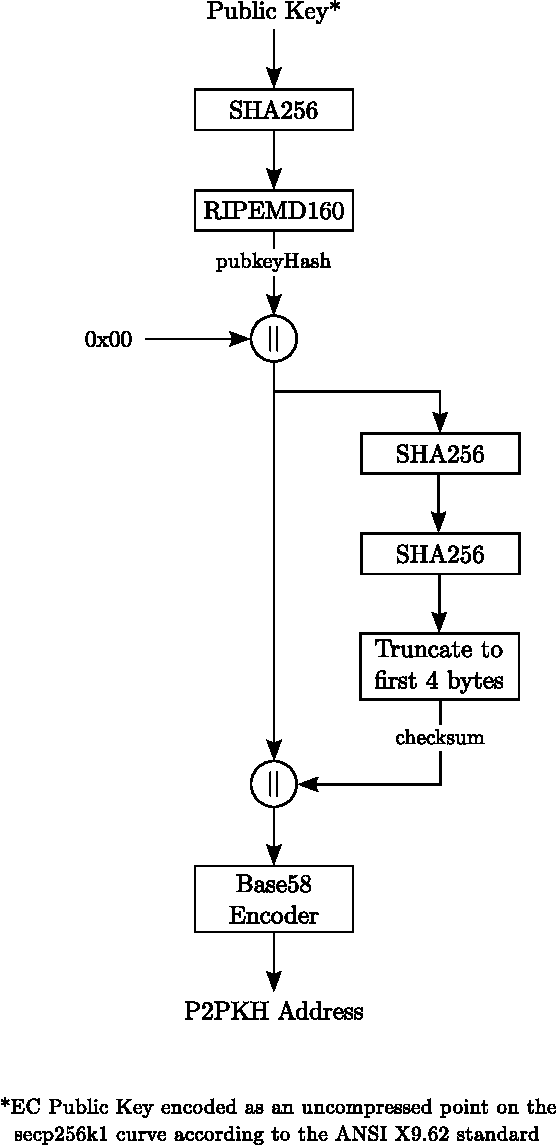
\includegraphics[scale=0.9]{Images/BitcoinAddress-P2PKH.pdf}

\vspace{10pt}
\caption{P2PKH Address Computation}
\label{fig:BitcoinAddress-P2PKH}
\end{figure}
\vspace{-10pt}


\subsubsection{Pay-to-ScriptHash Address} \label{sec:Address-P2SH}
A Pay-to-ScriptHash address on the other hand, is a hash of the redemption script \textit{serializedScript}, with a built-in checksum. Schematics of how it is calculated can be seen in Fig. \ref{fig:BitcoinAddress-P2SH}.~\\

\noindent
First, the redemption script is hashed using SHA256 and RIPEMD160. The resulting structure is referred to as \textit{scriptHash}. Next, a constant version byte is prepended to \textit{scriptHash}. A checksum is built over it by applying a double-SHA256 hash and truncating the result to the first 4 bytes. The checksum is then appended. Finally, the result is converted into a human-readable string using Base58 encoding \cite{Base58}. The final result is a \emph{P2SH address}.

\begin{figure}[htbp]

\centering
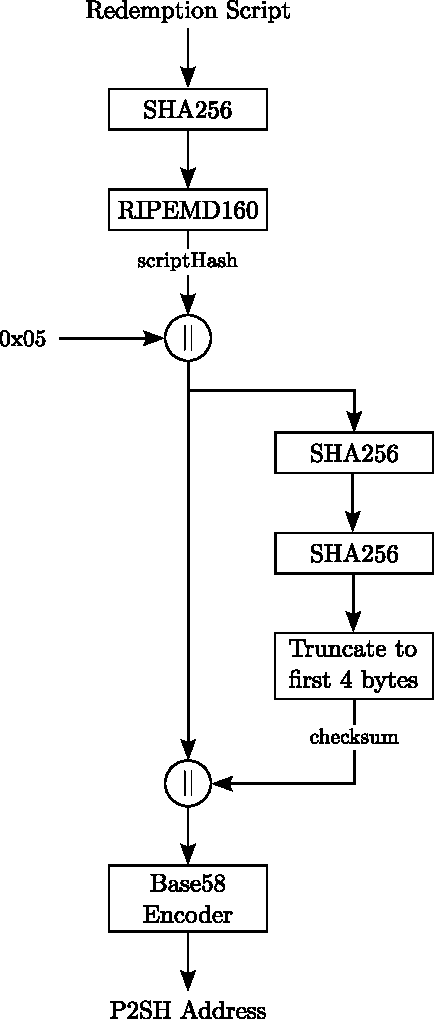
\includegraphics[scale=0.9]{Images/BitcoinAddress-P2SH.pdf}

\vspace{10pt}
\caption{P2SH Address Computation}
\label{fig:BitcoinAddress-P2SH}
\end{figure}
\vspace{-10pt}


\clearpage
\subsection{Signatures} \label{sec:Signatures}
Signatures are a central cryptographic primitive in Bitcoin and play a significant role in transaction authorization (see Sect. \ref{sec:OwnershipGeneral}). In a regular transaction, a signature is included in the signature script field (\textit{scriptSig}) of every transaction input to prove that the referenced transaction output can be rightfully spent by the claimant.

\subsection*{Hash Types}
Signatures in Bitcoin are of a specific type, referred to as \emph{hash type}, that determines which parts of the transaction are covered by it. This allows the signer to selectively choose which transaction parts should be protected and which parts can be modified by others. Three base signature hash types available, the default type \emph{SIGHASH\_ALL}, \emph{SIGHASH\_SINGLE} and \emph{SIGHASH\_NONE}. Additionally, a special type modifier called \emph{SIGHASH\_ANYONECANPAY} can be applied in conjunction with one of the three base types.

\vspace{-5pt}
\begin{figure}[ht!]
 \centering
 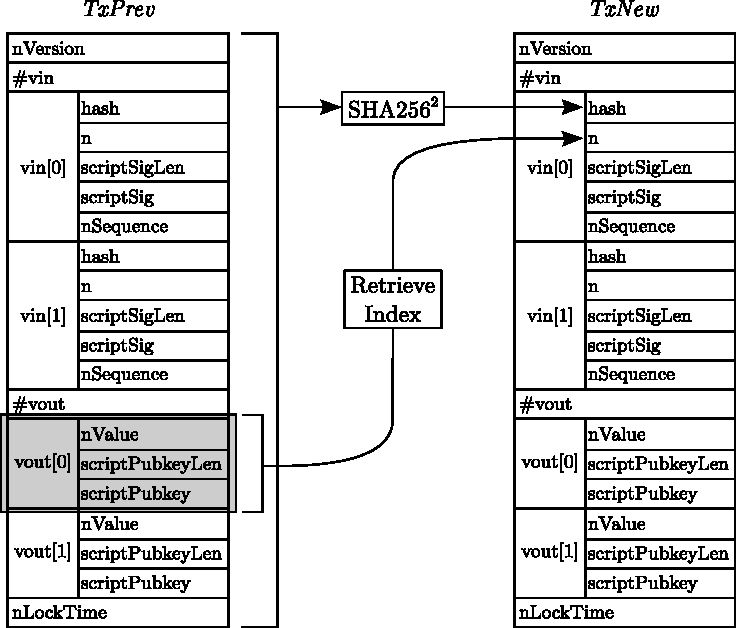
\includegraphics[scale=0.975]{Images/Transaction2In2Out.pdf}
 \caption{Signature Computation - Initial State} \label{fig:Signature-InitState}
\end{figure}
\vspace{-5pt}

\noindent
In the following the various signature types will be discussed in detail. The depiction in Fig. \ref{fig:Signature-InitState} shows the initial state of a sample transaction which will be used to illustrate the process. The signature will be performed for the first transaction input of the transaction \emph{TxNew}, which references the first output of a past transaction \emph{TxPrev}.

\clearpage
\subsection*{SIGHASH\_ALL}
The default signature hash type \emph{SIGHASH\_ALL} represents the simplest of the three base types. It signs the complete transaction, including all the transactions inputs and outputs, with the exception of the signature script fields. The coverage of the signature is illustrated below in Fig. \ref{fig:SigHash-All} with grey fields.

\begin{figure}[ht!]
 \centering
 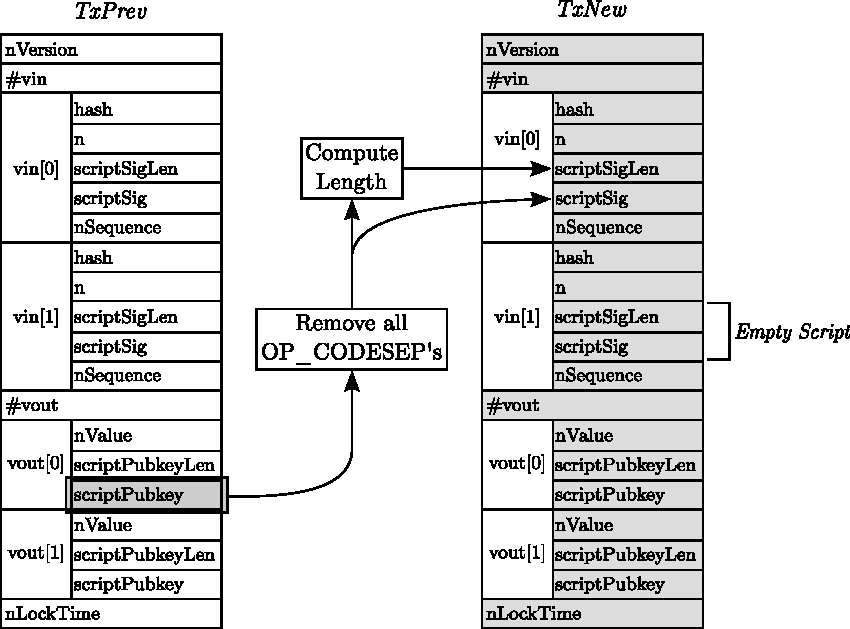
\includegraphics[scale=0.975]{Images/SIGHASH_ALL.pdf}
 \caption{Signature Computation - SIGHASH\_ALL} \label{fig:SigHash-All}
\end{figure}

\noindent
Before the signature is computed, several temporary changes are made to the transaction:
\begin{enumerate}[label=\alph*), leftmargin=1cm]
\item The signature script of the currently signed input is replaced with the public key script, excluding all occurences of \texttt{OP\_CODESEPARATOR} in it, of the referenced transaction output.
\item The signature scripts of all other inputs are replaced with empty scripts.
\end{enumerate}


\clearpage
\subsection*{SIGHASH\_SINGLE}
In the second signature hash type \emph{SIGHASH\_SINGLE} all transaction inputs and the transaction output corresponding to the currently signed input is signed. The coverage of the signature is illustrated below in Fig. \ref{fig:SigHash-Single} with grey fields.

\begin{figure}[ht!]
 \centering
 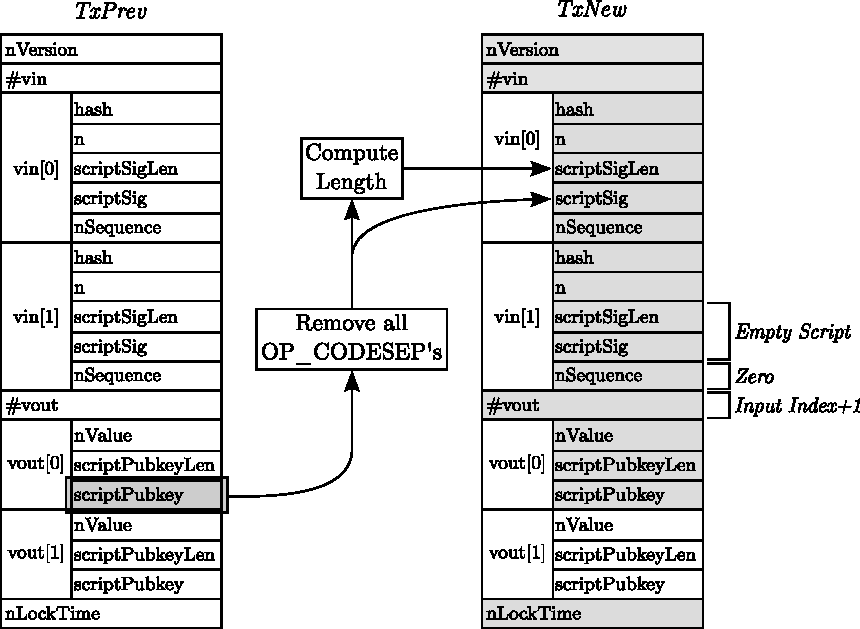
\includegraphics[scale=0.975]{Images/SIGHASH_SINGLE.pdf}
 \caption{Signature Computation - SIGHASH\_SINGLE} \label{fig:SigHash-Single}
\end{figure}

\noindent
Before the signature is computed, several temporary changes are made to the transaction:
\begin{enumerate}[label=\alph*), leftmargin=1cm]
\item The signature script of the currently signed input is replaced with the public key script, excluding all occurences of \texttt{OP\_CODESEPARATOR} in it, of the referenced transaction output.
\item For all the remaining transaction inputs:\vspace{5pt}
\begin{itemize}
\item[-] The signature scripts are replaced with empty scripts.
\item[-] The sequence number is set to zero.
\end{itemize}
\item The number of transaction outputs is set to the currently signed transaction input index plus one.
\item All transaction outputs up to the currently signed one are emptied.
\end{enumerate}


\clearpage
\subsection*{SIGHASH\_NONE}
In the third signature hash type \emph{SIGHASH\_NONE} all transaction inputs and none of the transaction outputs are signed. The coverage of the signature is illustrated below in Fig. \ref{fig:SigHash-None} with grey fields.

\begin{figure}[ht!]
 \centering
 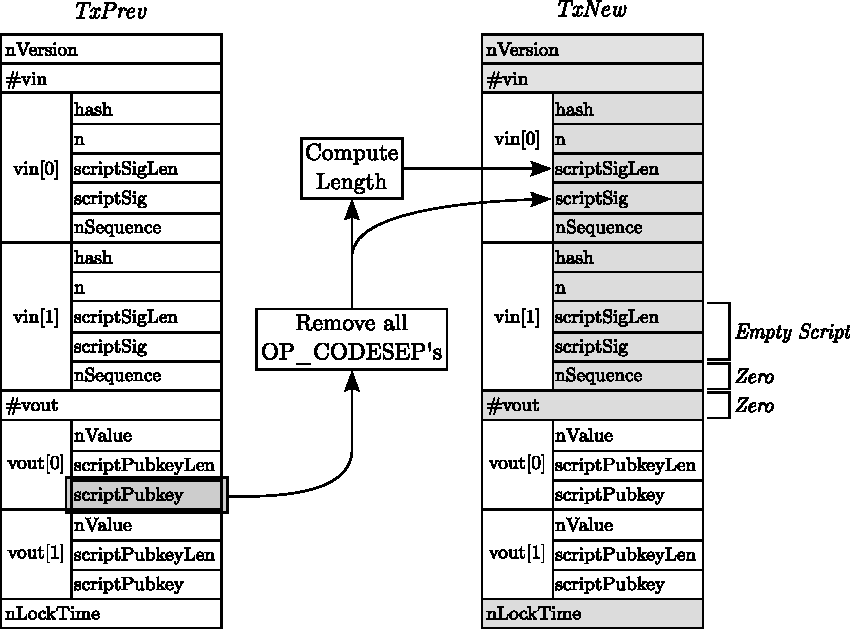
\includegraphics[scale=0.975]{Images/SIGHASH_NONE.pdf}
 \caption{Signature Computation - SIGHASH\_NONE} \label{fig:SigHash-None}
\end{figure}

\noindent
Before the signature is computed, several temporary changes are made to the transaction:
\begin{enumerate}[label=\alph*), leftmargin=1cm]
\item The signature script of the currently signed input is replaced with the public key script, excluding all occurences of \texttt{OP\_CODESEPARATOR} in it, of the referenced transaction output.
\item For all the remaining transaction inputs:\vspace{5pt}
\begin{itemize}
\item[-] The signature scripts are replaced with empty scripts.
\item[-] The sequence number is set to zero.
\end{itemize}
\item The number of transaction outputs is set to zero.
\item All transaction outputs are removed.
\end{enumerate}


\clearpage
\subsection*{SIGHASH\_ANYONECANPAY}
The \emph{SIGHASH\_ANYONECANPAY} modifier is used in conjunction with a base type and affects the signature coverage of transaction inputs. It is used to only cover the currently signed input by the signature. For example, the transaction depicted in Fig. \ref{fig:SigHash-Anyone} illustrates that the second transaction input is excluded from the signature.

\begin{figure}[ht!]
 \centering
 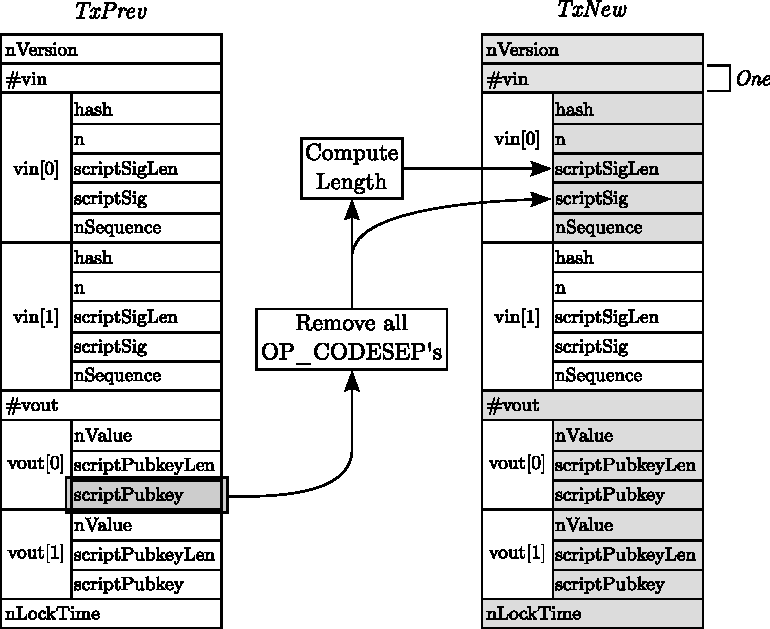
\includegraphics[scale=0.975]{Images/SIGHASH_ANYONECANPAY.pdf}
 \caption{Signature Computation - SIGHASH\_ALL\textbar SIGHASH\_ANYONECANPAY} \label{fig:SigHash-Anyone}
\end{figure}

\noindent
In addition to the changes performed by the base hash type, the following temporary changes are made before the signature is computed:
\begin{enumerate}[label=\alph*), leftmargin=1cm]
\item The number of transaction inputs is set to one.
\item All transaction inputs, except for the currently signed one, are removed.
\end{enumerate}

\clearpage
\subsection*{Finalization}
Once the transaction type has been chosen and the hash type dependent modifications have been applied, the actual signature is computed. This is done as follows - first, the hash type is appended to the transaction, then the signature itself is computed and finally the hashtype is appended to it. The ECDSA signature is computed using double-SHA256 and the secp256k1 elliptic curve as parameters. The appended hashtype signals the verifying party what hash type was applied.

\begin{figure}[ht!]
 \centering
 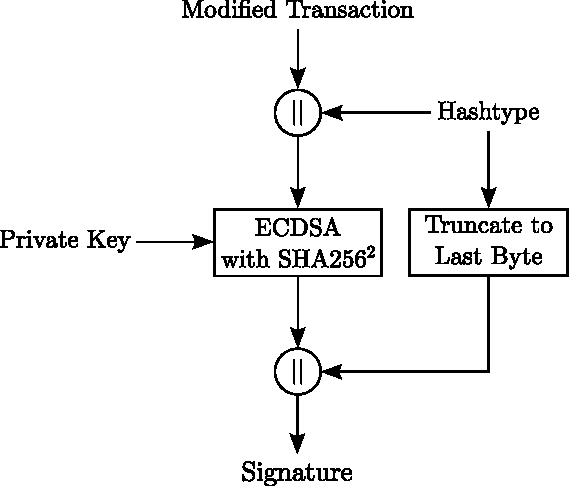
\includegraphics[scale=0.9]{Images/Signature-Finalization.pdf}
 
 \vspace{5pt}
 \caption{Signature Computation - Finalization} \label{fig:SigFin-SighashAll}
\end{figure}